\let\negmedspace\undefined
\let\negthickspace\undefined
\documentclass[journal]{IEEEtran}
\usepackage[a5paper, margin=10mm, onecolumn]{geometry}
%\usepackage{lmodern} % Ensure lmodern is loaded for pdflatex
% \usepackage{tfrupee} % Include tfrupee package

\setlength{\headheight}{1cm} % Set the height of the header box
\setlength{\headsep}{0mm}     % Set the distance between the header box and the top of the text

\usepackage{gvv-book}
\usepackage{gvv}
\usepackage{cite}
\usepackage{amsmath,amssymb,amsfonts,amsthm}
\usepackage{algorithm}
\usepackage{algorithmic}
\usepackage{graphicx}
\usepackage{textcomp}
\usepackage{xcolor}
\usepackage{txfonts}
\usepackage{listings}
\usepackage{enumitem}
\usepackage{mathtools}
\usepackage{gensymb}
\usepackage{comment}
\usepackage[breaklinks=true]{hyperref}
\usepackage{tkz-euclide} 
\usepackage{listings}
% \usepackage{gvv}                                        
\def\inputGnumericTable{}                                 
\usepackage[latin1]{inputenc}                                
\usepackage{color}                                            
\usepackage{array}                                            
\usepackage{longtable}                
\usepackage{calc}                                             
\usepackage{multirow}                                         
\usepackage{hhline}                                           
\usepackage{ifthen}                             
\usepackage{caption}              
\usepackage{lscape}
\usepackage{subcaption}
\captionsetup{compatibility=false}
% \captionsetup{compactibility=false}
% \usepackage{algpseudocode}
\begin{document}

\bibliographystyle{IEEEtran}
\vspace{3cm}

\title{Experiment 3} 
\author{S A Aravind Eswar and Eshan Sharma}
{\let\newpage\relax\maketitle}

\section{Aim}

Study and plot Bode plot of magnitude and phase response for 1-stage, 2-stage, 3-stage RC Low pass filter.

\section{Materials and Apparatus Required}

\begin{enumerate}
    \item 3 Reistors (1k$\Omega$ used)
    \item 3 Capasitors (0.1$\mu$F used)
    \item Bread Board
    \item Function Generator
    \item Oscilloscope
\end{enumerate}

\section{Theory}

The transfter function of a 1-stage RC circuit would be the following,

\begin{align*}
    \vec{H(s)} = \frac{1}{1+sRC}
\end{align*}

where,

\begin{align*}
    s = j\omega
\end{align*}
expanding, we get,

\begin{align*}
    \vec{H(s)} = \frac{1}{\sqrt{1+(\omega RC)^2}} e^{j\theta}
\end{align*}
where,
\begin{align*}
    \theta = \tan^{-1}\brak{-\omega RC}
\end{align*}

Applying logarithm on both sides, we get,

\begin{align*}
    \log{\vec{H(s)}} &= \log\brak{\frac{1}{\sqrt{1+(\omega RC)^2}} e^{j\tan^{-1}\brak{-\omega RC}}}\\
                  &= -\frac{1}{2}\log\brak{1+(\omega RC)^2} + j \tan^{-1}\brak{-\omega RC}
\end{align*}

Calculating Amplitude gain,

\begin{align*}
    A &= 20 \log\brak{\abs{\vec{H(s)}}}\\
    A &= -10 \log\brak{1+\brak{\omega RC}^2}
\end{align*}

This gives the exact equation for Bode plot of the amplitude gain.

For phase difference,

\begin{align*}
    \theta &= 20\tan^{-1}\brak{-\omega RC}
\end{align*}

% when, $1 >> \brak{\omega RC}$
% From this, we can infer that the real part gives the Bode equation for the amplitude and imaginary part gives the equation for phase.

Similarly,

The transfer function of 2-stage RC circuit would be,

\begin{align*}
    \vec{H(s)} = \brak{\frac{1}{1-\brak{\omega RC}^2 + 3sRC}}
\end{align*}

And following this, we get,

\begin{align*}
    \log\vec{H(s)} = -\frac{1}{2}\log\brak{(1-(\omega RC)^2)^2 + (3\omega RC)^2} + j \tan^{-1}\brak{\frac{-3\omega RC}{1-(\omega RC)^2}}
\end{align*}

And,

The transfer function for 3-state RC circuit is given as,

\begin{align*}
    \vec{H(s)} = \brak{\frac{1}{\brak{sRC}^3+5\brak{sRC}^2+6sRC+1}}
\end{align*}

And following that we get,

\begin{align*}
    \log{\vec{H(s)}} = -\frac{1}{2}\log\brak{\brak{1-5\brak{\omega RC}^2}^2+\brak{6\omega RC - \brak{\omega RC}^3}} + j \tan^{-1}\brak{-\omega RC\frac{6-\brak{\omega RC}^2}{1-5\brak{\omega RC}^2}}
\end{align*}

\section{Procedure}

\begin{figure}[!ht]
    \centering
    \resizebox{0.7\textwidth}{!}{%
    \begin{circuitikz}
    \tikzstyle{every node}=[font=\normalsize]
    % \draw (4.75,14.5) to[R] (4.75,14.5);
    \draw (4.75,14.5) to[R] (7.25,14.5);
    \draw (7.25,14.5) to[R] (10.5,14.5);
    \draw (10.5,14.5) to[R] (13,14.5);
    \draw (7.5,14.5) to[C] (7.5,12);
    \draw (10.25,14.5) to[C] (10.25,12);
    \draw (13,14.5) to[C] (13,12);
    \draw (13,12) to[short] (4.75,12);
    \draw (4.75,14.5) to[short, -o] (4.5,14.5) ;
    \draw (4.75,12) to[short, -o] (4.5,12) ;
    \node at (7.5,14.5) [circ] {};
    \node at (7.5,12) [circ] {};
    \node at (10.25,12) [circ] {};
    \node at (10.25,14.5) [circ] {};
    \node at (13,14.5) [circ] {};
    \node at (13,12) [circ] {};
    \node [font=\normalsize] at (7.5,14.75) {A};
    \node [font=\normalsize] at (7.5,11.75) {A'};
    \node [font=\normalsize] at (10.25,11.75) {B'};
    \node [font=\normalsize] at (10.25,14.75) {B};
    \node [font=\normalsize] at (13,14.75) {C};
    \node [font=\normalsize] at (13,11.75) {C'};
    \end{circuitikz}
    }%
    \caption{Circuit Diagram}
    \label{fig:my_label}
\end{figure}

\begin{enumerate}
    \item Make connections as given in fig. \ref{fig:my_label}
    \item Give input $\vec{V{in}}$ in the open end.
    \item Measure Voltage across $A-A'$ and Phase difference between input voltage and output voltage for 1 cascade circuit analysis.
    \item Record observations for multiple input frequencies.
    \item Repeat the experiment for $B-B'$ and $C-C'$ for 2 cascade and 3 cascade circuit analysis respectively.
    \item Compare the theoreical caltuations and observed values.
\end{enumerate}

\section{Observations}

\begin{table}[h]
    \centering
    \begin{tabular}{| m{5em} | m{5 em} |m{5em}|}
    \hline
    $f$ & $V_{out}$ & $\Delta t$\\
    \hline
    $10 Hz$ & 5.001$V$ & $5.6 ms$\\
    $100 Hz$ & $5.001 V$ & $560 \mu s$\\
    $500 Hz$ & $5.001 V$ & $300 \mu s$\\
    $1000 Hz$ & $3.201 V$ & $96 \mu s$\\
    $5000 Hz$ & $1.441 V$ & $31.2 \mu s$\\
    $10k Hz$ & $880 mV$ & $18.4 \mu s$\\
    $50k Hz$ & $200 mV$ & $4.48 \mu s$\\
    $100kHz$ & $104 mV$ & $2.2 \mu s$\\
    $500kHz$ & $30 mV$ & --\\
    $1MHz$ & $16mV$ & --\\
    \hline
    
\end{tabular}
    \caption{Obsereved 1 Cascade Circuit Response}
\end{table}

\begin{table}[h]
    \centering
    \begin{tabular}{| m{5em} | m{5em} | m{5em} |}
    \hline
    $f$ & $V_{out}$ & $\Delta t$\\
    \hline
    $10Hz$ & $5.001V$ & $5.2 ms$\\
    $50Hz$ & $5.001V$ & $520 \mu s$\\
    $100Hz$ & $5.001V$ & $320 \mu s$\\
    $500Hz$ & $4.401V$ & $216 \mu s$\\
    $1kHz$ & $3.001V$ & $184\mu s$\\
    $5kHz$ & $580mV$ & $68 \mu s$\\
    $10kHz$ & $184mV$ & $40 \mu s$\\
    $50kHz$ & $16mV$ & $10.8\mu s$\\
    \hline
\end{tabular}
    \caption{Obsereved 2 Cascade Circuit Response}
\end{table}

\begin{table}[h]
    \centering
    \begin{tabular}{| m{5em} | m{5em} | m{5em} |}
    \hline
    $f$ & $V_{out}$ & $\Delta t$\\ 
    \hline
    $10Hz$ & $4.601V$ & $1.6ms$\\
    $50Hz$ & $5.001V$ & $200\mu s$\\
    $100Hs$ & $5.001V$ & $220\mu s$\\
    $1kHz$ & $3.001V$ & $176\mu s$\\
    $5kHz$ & $120mV$ & --\\
    $10kHz$ & $30mV$ & --\\
    \hline
\end{tabular}
    \caption{Observed 3 Cascade Circuit Response}
\end{table}

\begin{figure}[h]
    \centering
    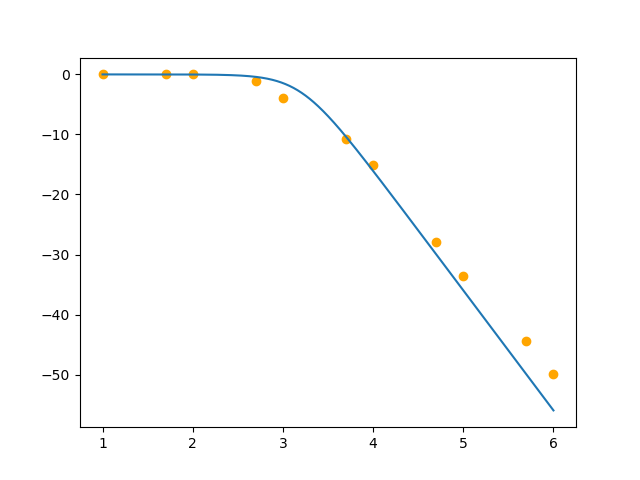
\includegraphics[width=0.7\columnwidth]{figs/Afig1.png}
    \caption{Amplitude graph for 1 cascase response}
\end{figure}

\begin{figure}[h]
    \centering
    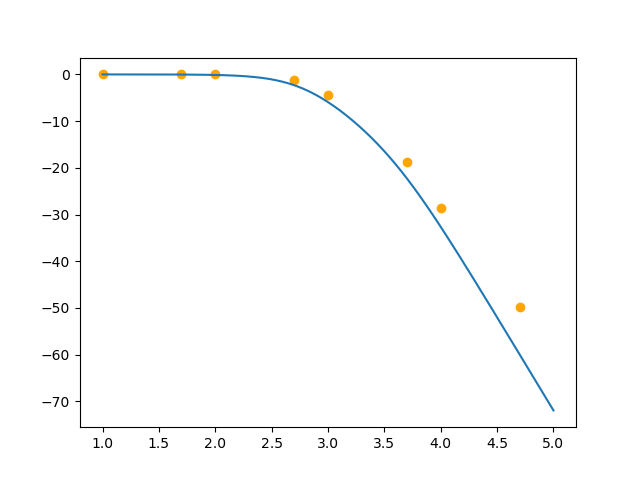
\includegraphics[width=0.7\columnwidth]{figs/Afig2.png}
    \caption{Amplitude graph for 2 cascase response}
\end{figure}

\begin{figure}[h]
    \centering
    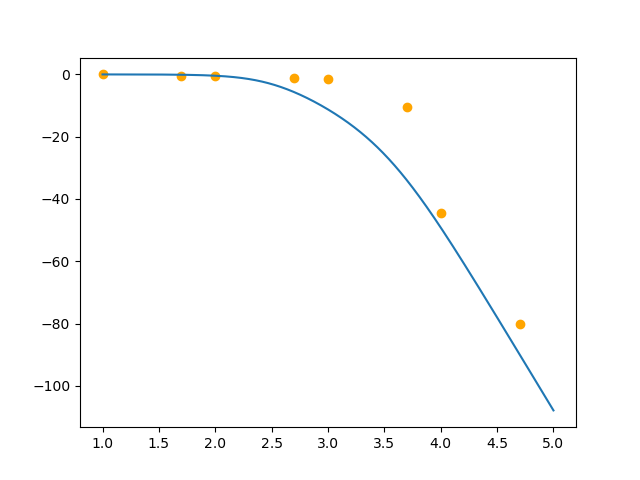
\includegraphics[width=0.7\columnwidth]{figs/Afig3.png}
    \caption{Amplitude graph for 3 cascase response}
\end{figure}

\begin{figure}[h]
    \centering
    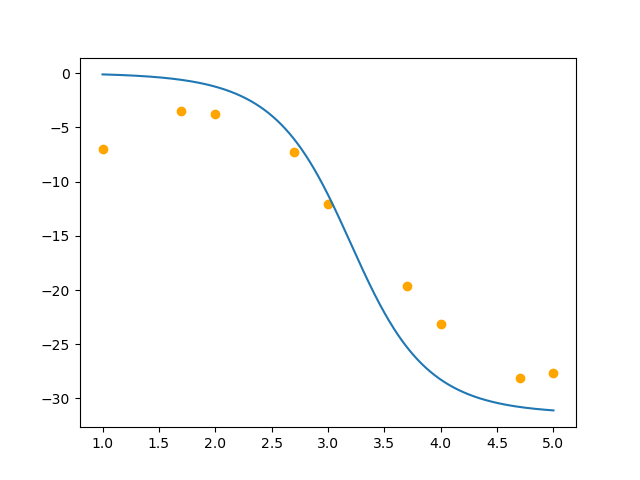
\includegraphics[width=0.7\columnwidth]{figs/Pfig1.png}
    \caption{Phase graph for 1 cascase response}
\end{figure}

\begin{figure}[h]
    \centering
    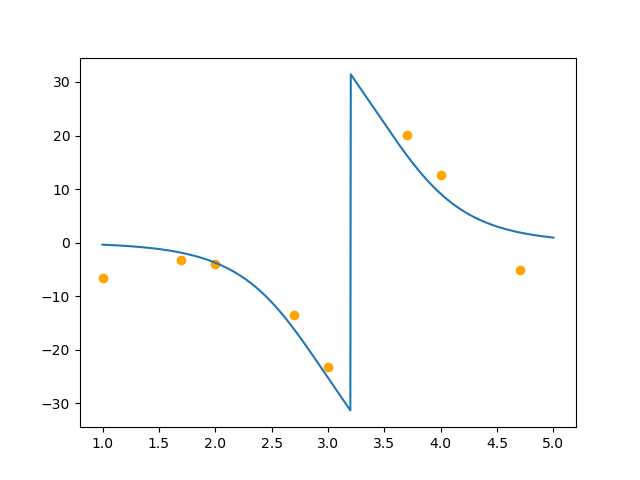
\includegraphics[width=0.7\columnwidth]{figs/Pfig2.png}
    \caption{Phase graph for 2 cascase response}
\end{figure}

\begin{figure}[h]
    \centering
    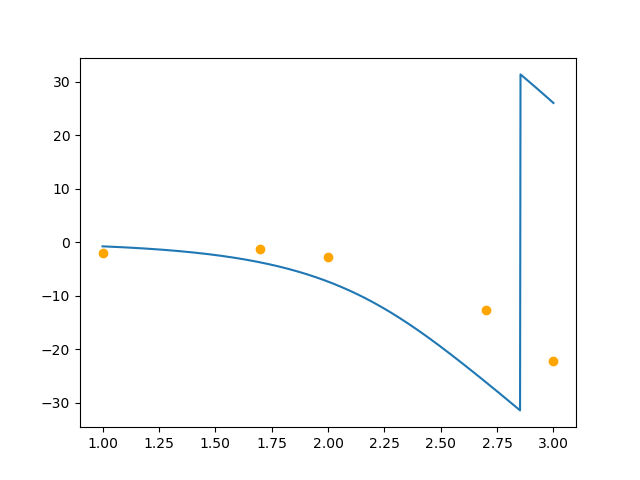
\includegraphics[width=0.7\columnwidth]{figs/Pfig3.png}
    \caption{Phase graph for 2 cascase response}
\end{figure}

\end{document}
